\documentclass[12pt]{../notes}

% Command for Questions
%\question{}

% Command for Notes
% \note{}

% Code to create a minipage where you can type in class notes. 
%%\begin{minipage}[l][2cm][c]{\textwidth}
%\begin{comment}

%\end{comment}
%%\end{minipage}

%\usepackage{listings}

% In order for the minted code to run, we had to create a new compilation routine called pdflatex+shellEscape.
% This includes a --shell-escape command which should ONLY be used when pygmentized is required as it compromises security. 
% We also had to add pygmentize (a python package) to the system path (BEFORE miktex) and then restart the computer. 
%\usepackage{minted}
%\usemintedstyle{borland}
%\lstset{language=SAS, 
 % breaklines=true,  
 % basicstyle=\ttfamily\bfseries,
  %columns=fixed,
  %keepspaces=true,
  %identifierstyle=\color{blue}\ttfamily,
  %keywordstyle=\color{cyan}\ttfamily,
  %stringstyle=\color{purple}\ttfamily,
  %commentstyle=\color{green}\ttfamily,
  %} 
  
% \begin{minted}{sas}
% \end{minted}

\usepackage{hyperref}


% Begin Document
%==============================================================================
\begin{document}
% Include the Title of the Handout
\ntitle{7.2: Principal Components and Quantile Regression}

\section{Principal Components (PC) Regression}
\begin{figure}[H]
\centering
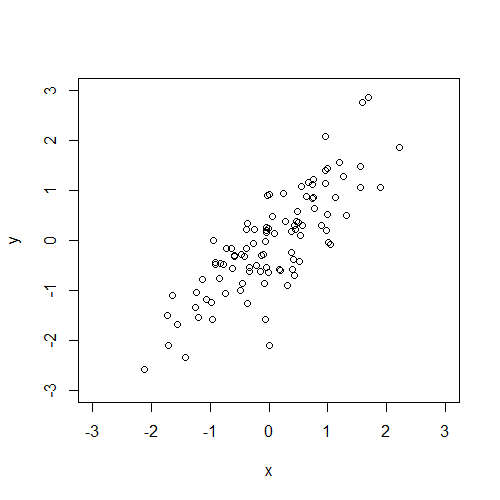
\includegraphics[width=0.4\textwidth]{../figures/module7/pc_scatter.png}
\end{figure}

\section{Principal Components (PC) Regression}
\textbf{Principal Components} is essentially a \textbf{re-projection} of the data into a new space where each axis follows the direction of the \textbf{highest variance} of the data, in descending order. 
\bi
\item Each component is a linear combination of the original $X$ variables. 
\begin{align*}
PC_{i, 1} &= a_1^{(1)}X_{i, 1} + \cdots + a^{(1)}_{p-1}X_{i, p-1} \\
PC_{i, 2} &= a_1^{(2)}X_{i, 1} + \cdots + a^{(2)}_{p-1}X_{i, p-1} \\
& \vdots \\
PC_{i, p-1} &= a_1^{(p-1)}X_{i, 1} + \cdots + a^{(p-1)}_{p-1}X_{i, p-1} \\
\end{align*}
\item Components derived from eigenvalues/eigenvectors of the matrix $X^TX$
\item Often used as a form of dimensionality reduction. 
\ei

Nice Mathematical Properties:
\bi
\item $\rho(PC_j, PC_k) = 0 \quad \forall j \ne k$
\item $\sum_j\left(a_j^{(k)}\right)^2 = 1$
\item $Var(PC_1) \ge Var(PC_2) \ge \cdots \ge Var(PC_{p-1})$
\ei

\subsection{Model}
$$Y_i = \beta_0 + \beta_1PC_{i, 1} + \cdots + \beta_{p-1}X_{i, p-1} + \epsilon_i$$
estimated with 
$$\hat{Y}= \beta_0 + b_1PC_{i, 1} + \cdots + b_{p-1}X_{i, p-1}.$$

\textbf{Note:} The PC's only consider relationships among the X variables and do not depend on Y. 

\nspace
\textbf{Consequently,} \textit{all} of the principal components should be considered, not just the first few. 

\question{Why might dropping ``low variance'' principal components hurt our regression model?}

% Code to create a minipage where you can type in class notes. 
\begin{minipage}[l][2cm][c]{\textwidth}
%\begin{comment}
\note{Because the principal components have nothing to do with Y, its possible that a ``low variance'' combination of the X-variables is highly correlated with Y.}
%\end{comment}
\end{minipage}

\subsection{Pros and Cons}
\bi
\item \textbf{Pro:} Guaranteed uncorrelated predictors $\rightarrow$ no multicollinearity $\rightarrow$ meaningful model \textit{coefficients}. 
\item \textbf{Con:} No guarantee of meaningful \textit{variables.}
\ei

\begin{comment}
\begin{minted}{sas}
proc princomp data=<dataset> standard out=<output dataset>;
var <all x variables>;
run;

proc reg data=PCout;
  model <y-variable> = Prin1-Prin<lastnumber> / vif;
run;
\end{minted}
\end{comment}

\section{Quantile Regression}
Quantiles: a set of $q$ ranges for which there is an equal probability of an observation falling into each range. 
\bi
\item Example: the median splits the observations into two groups, where 50\% of the observations fall in each group. 
\ei

In ordinary least squares (OLS) our goal was to model the \textbf{mean} of the response variable Y. 
$$E\{Y\} = \beta_0 + \beta_1X_1 + \cdots + \beta_{p-1}X_{p-1}$$
with 
$$\hat{Y} = b_0 + b_1X_1 + \cdots + b_{p-1}X_{p-1}$$
based on the assumption that the model residuals were unbiased, normally distributed, with constant variance. 

\nspace
If the variance was not constant across $Y$, we were forced to consider variable transformations (Handout 2.2) or weighted least squares regression (Handout 4.2). 

\nspace
In quantile regression, heterskedasticity is seen as an \textbf{opportunity} to be pursued, rather than a \textbf{problem} to be fixed. 

\subsection{Motivating Example}
\question{Looking at Figure \ref{fig:edscatter}, how does the relationship between a Husband's education level and income change \textit{across the quantiles of income}? }

\begin{figure}[H]
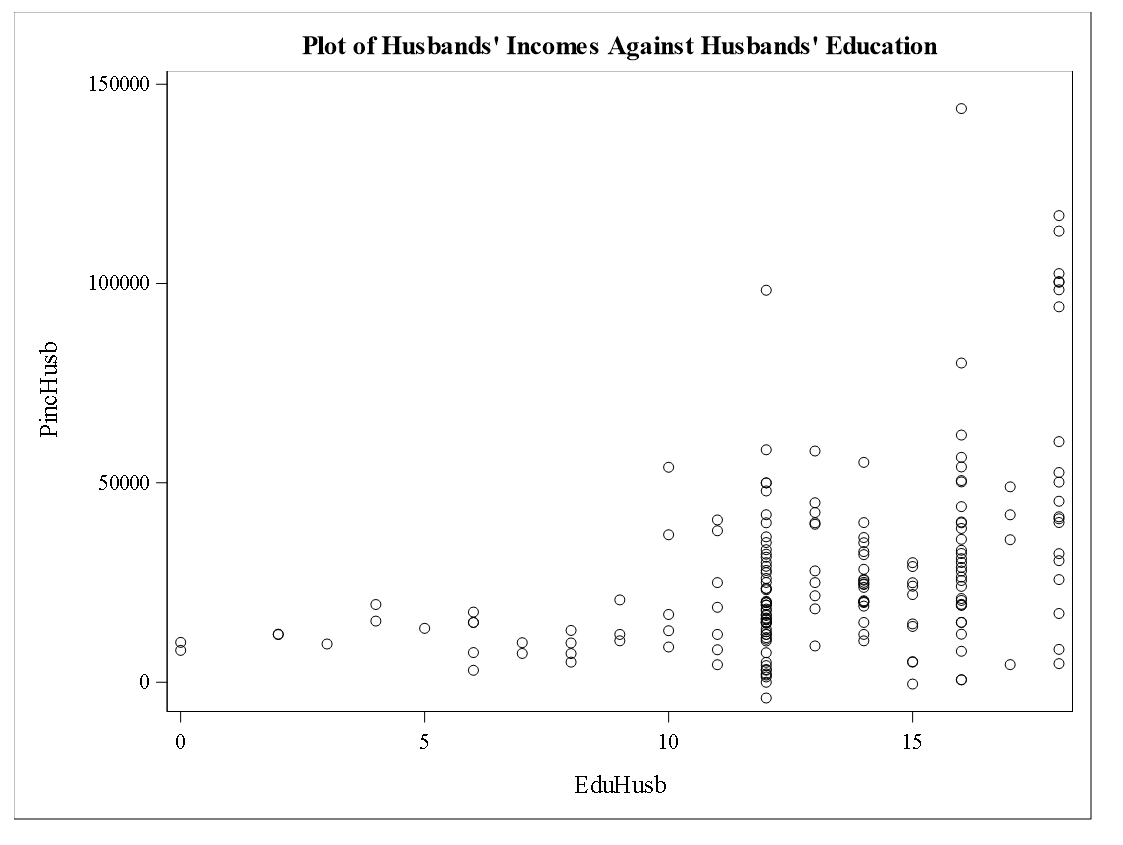
\includegraphics[width=0.48\textwidth]{../figures/module7/education_scatter.png}
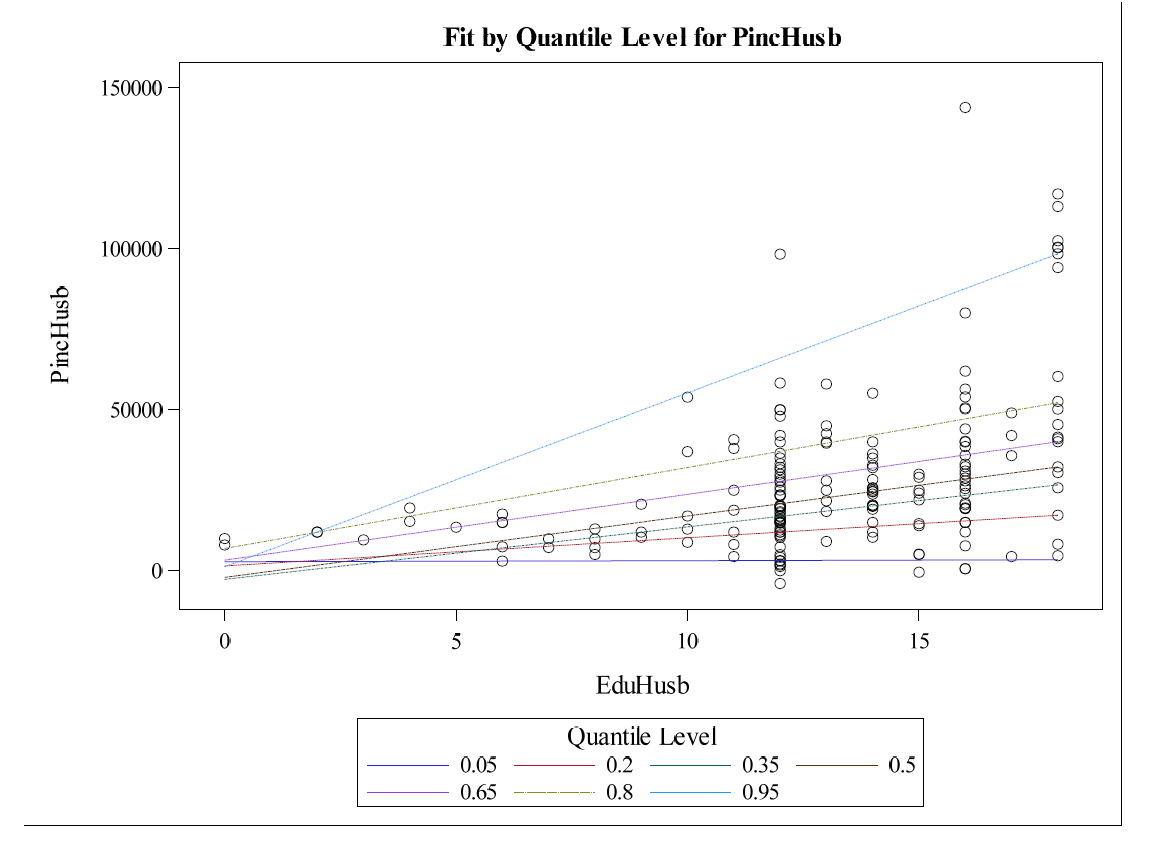
\includegraphics[width=0.48\textwidth]{../figures/module7/education_scatter_2.png}
\caption{(Left) Plot of education vs income level. (Right) Series of quantile regression lines overlaid on the scatterplot of education and income.}
\label{fig:edscatter}
\end{figure}

\begin{minipage}[l][2cm][c]{\textwidth}
%\begin{comment}
\note{Notice that the positive association between education and income level is much more drastic when comparing only high income earners in each educational group. }
%\end{comment}
\end{minipage}

\nspace 
Simply trying to model effect of education on \textit{average} income doesn't tell the full story. 

\subsection{Model}
In ordinary least squares (OLS) regression, we assume the model 

$$Y_i = \beta_0 + \beta_1X_{i, 1} + \cdots + \beta_{p-1}X_{i, p-1} + \epsilon_i$$ where estimated coefficients $b_j$ were selected to minimize $\sum_i\left(Y_i - \hat{Y}_i\right)^2.$

\nspace
In contrast, Quantile Regression selects $b_k(\tau)$ to minimize $\sum_i\rho_\tau\left(Y_i - Q_\tau(Y_i)\right)$, where
$$Q_\tau(Y_i) = b_0(\tau) + b_1(\tau)X_{i, 1} + \cdots + b_{p-1}(\tau)X_{i, p-1}$$
\begin{tabular}{ll}
$\tau$ & a quantile from 0 to 1 \\
$b_j(\tau)$ & estimated coefficient (a function of the quantile) \\
$Q_\tau(Y_i)$ & the estimated $\tau$ quantile for the X-profile $X_{i, 1}, \ldots, X_{i, p-1}$ \\
$\rho_\tau(r)$ & a ``check loss'' function $\rho_\tau(r) = \text{max}\{\tau r, (\tau - 1)r\}$
\end{tabular}

\question{For the check loss function in Figure \ref{fig:checkloss}, X is the value of the residual and Y is the penalty associated with the residual. Knowing this, how do the ``penalties'' for $\tau = 0.3$ and $\tau = 0.9$ differ? Why does this difference seem reasonable?}

% Code to create a minipage where you can type in class notes. 
\begin{minipage}[l][3cm][c]{\textwidth}
%\begin{comment}
\note{For $\tau = 0.9$ an over-prediction is not penalized nearly as much as an under-prediction. The opposite is true for $\tau = 0.3.$ This makes sense because we would expect most of the points to be above the $\tau = 0.3$ line, and below the $\tau = 0.9$ line.}
%\end{comment}
\end{minipage}

\begin{figure}[H]
\centering
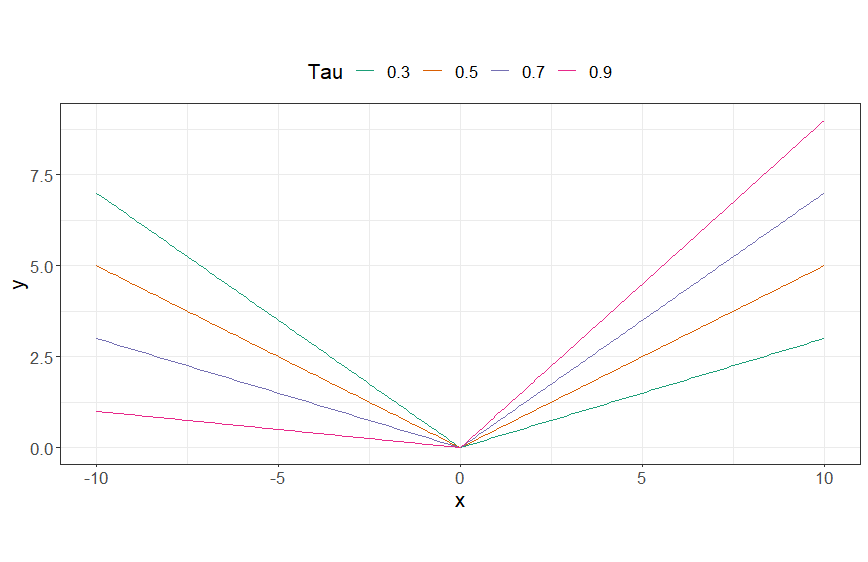
\includegraphics[width=0.75\textwidth]{../figures/module7/checkloss.png}
\caption{Check loss functions for various quantiles.}
\label{fig:checkloss}
\end{figure}

\subsection{Comparison to OLS}
\begin{tabular}{|p{9cm}|p{9cm}|}
\hline
\textbf{OLS} & \textbf{Quantile Regression} \\ 
\hline
Predicts conditional mean $E(Y|X_1, X_2, \ldots)$ & Predicts conditional \textit{distribution} (via quantiles) \\
& \\
Error terms must meet distributional assumptions & No assumptions for error terms \\
& \\
Sensitive to outliers  & Robust to outliers (except extreme quantiles) \\
& \\
Effectively applied to small samples & Data-hungry \\
& \\
Computationally cheap & Computationally expensive (no closed-form solution/requires lots of quantile models). \\
\hline
\end{tabular}

\begin{comment}
\subsection{SAS Code}
\begin{minted}{sas}
proc quantreg data=<dataset>;
model <model statement> /
quantile= <low> to <high> by <increment>
plot=quantplot;
run;

proc quantselect data=<dataset> plots=coefficients;
model <model statement>
/ quantile = 0.1 0.5 0.9 selection=lasso(sh=<step horizon (integer)>);
partition fraction(validate=0.3);
run;
\end{minted}
\end{comment}








\subsection{Good Resources}
\bi
\item Rodriguez, Bob and Yao, Yonggang (2017) “Five Things You Should Know About Quantile Regression” \url{https://support.sas.com/resources/papers/proceedings17/SAS0525-2017.pdf} 
\item Rodriguez, Bob (2018) “Three Things you Should Know About Quantile Regression” \url{https://www.youtube.com/watch?v=CU0ofd3hSOA} 
\ei
% End the Document
%==============================================================================
\end{document}